\subsection{\texorpdfstring{\(E_{8}\) 型系统}{E\_8 型系统}}

\begin{enumerate}
\def\labelenumi{(\Roman{enumi})}
\tightlist
\item
  考虑第 4 号的群 \(\mathbf{L}_3\)，它位于 \(\mathbf{R}^8\) 中。令 \(\mathbf{R}\) 为满足 \(\alpha \in \mathbf{L}_3\) 且 \((\alpha |\alpha) = 2\) 的向量集合；它包含向量
\end{enumerate}

\[
\pm \varepsilon_ {i} \pm \varepsilon_ {j} (i <   j). \frac {1}{2} \sum_ {i = 1} ^ {8} (- 1) ^ {\nu (\mathrm{i})} \varepsilon_ {i} \left(\sum_ {i = 1} ^ {8} \nu (i) \text {even}\right).
\]

反之，若元素 \(\alpha \in L_3\) 满足 \((\alpha |\alpha) = 2\)，则其坐标必须取自 \(0, \pm \frac{1}{2}, \pm 1\)；由第 4 号，这些坐标要么全为整数，从而得到向量 \(\pm \varepsilon_i \pm \varepsilon_j\)，要么全都等于 \(\pm \frac{1}{2}\) 且其和为整数，从而得到向量

\[
\frac {1}{2} \sum_ {i = 1} ^ {8} (- 1) ^ {\nu (\mathrm{i})} \varepsilon_ {i}
\]

其中 \(\sum_{i=1}^{8} \nu(i)\) 为偶数。

  由第 4 号知，\((\alpha |\beta)\in \mathbf{Z}\) 对所有 \(\alpha ,\beta \in \mathrm{L}_3\) 成立。因此，R 是约化根系。根的数目为 \(n = \binom{8}{2}.4 + 2^7 = 240\)

\begin{enumerate}
\def\labelenumi{(\Roman{enumi})}
\setcounter{enumi}{1}
\tightlist
\item
  令 \(\rho\) 为向量 \((0,1,2,3,4,5,6,23)\)，它属于 \(L_{3}\)。\(R\) 中没有元素与 \(\rho\) 正交（对 \(\pm \varepsilon_{i} \pm \varepsilon_{j}\) 显然如此；若 \(\frac{1}{2} \sum_{i=1}^{8} (-1)^{\nu(i)} \varepsilon_{i}\) 与 \(\rho\) 正交，则应有 \(\sum_{i=1}^{6} i(-1)^{\nu(i+1)} + 23(-1)^{\nu(8)} = 0\)，但这是不可能的，因为 \(\sum_{i=1}^{6} i < 23\)）。因此，根据（ \(\S\) 1，第 7 号，命题 20 的推论 2），满足 \(\alpha \in R\) 且 \((\alpha | \rho) > 0\) 的根是相对于某个室的正根。这些根是 \(\pm \varepsilon_{i} + \varepsilon_{j}\)（ \(i < j\)），以及
\end{enumerate}

\[
\frac {1}{2} \left(\varepsilon_ {8} + \sum_ {i = 1} ^ {7} (- 1) ^ {\nu (\mathrm{i})} \varepsilon_ {i}\right)
\]

  其中 \(\sum_{i=1}^{7} \nu(i)\) 为偶数。\((\alpha|\rho) \in \mathbf{Z}\) 对所有 \(\alpha \in \mathrm{R}\) 成立（第 4 号），且对于下列根，\((\alpha|\rho)\) 等于 1：

\[
\alpha_ {1} = \frac {1}{2} (\varepsilon_ {1} + \varepsilon_ {8}) - \frac {1}{2} (\varepsilon_ {2} + \varepsilon_ {3} + \varepsilon_ {4} + \varepsilon_ {5} + \varepsilon_ {6} + \varepsilon_ {7}),
\]

\[
\alpha_ {2} = \varepsilon_ {1} + \varepsilon_ {2}, \alpha_ {3} = \varepsilon_ {2} - \varepsilon_ {1}, \alpha_ {4} = \varepsilon_ {3} - \varepsilon_ {2}, \alpha_ {5} = \varepsilon_ {4} - \varepsilon_ {3},
\]

\[
\alpha_ {6} = \varepsilon_ {5} - \varepsilon_ {4}, \alpha_ {7} = \varepsilon_ {6} - \varepsilon_ {5}, \alpha_ {8} = \varepsilon_ {7} - \varepsilon_ {6}.
\]

这八个向量构成 \(R^{8}\) 的一个基。由 § 1，第 6 号，命题 19 的推论 1，\((\alpha_{1}, \alpha_{2}, \ldots, \alpha_{8})\) 是 R 的一个基，并且相对于此基的正根正是上面所定义的那些根。我们有

\[
\left(\alpha_ {4} \mid \alpha_ {5}\right) = \left(\alpha_ {5} \mid \alpha_ {6}\right) = \left(\alpha_ {6} \mid \alpha_ {7}\right) = \left(\alpha_ {7} \mid \alpha_ {8}\right) = \left(\alpha_ {4} \mid \alpha_ {2}\right) = \left(\alpha_ {4} \mid \alpha_ {3}\right) = \left(\alpha_ {3} \mid \alpha_ {1}\right) = - 1,
\]

且对所有其他指标对都有 \((\alpha_{i}|\alpha_{j})=0\)。因此，R 的 Dynkin 图为 \(E_{8}\) 型，且 R 不可约。

\begin{enumerate}
\def\labelenumi{(\Roman{enumi})}
\setcounter{enumi}{2}
\item
  我们有 \(h = \frac{n}{8} = 30\)。
\item
  令
\end{enumerate}

\[
\tilde {\alpha} = \varepsilon_ {7} + \varepsilon_ {8} = 2 \alpha_ {1} + 3 \alpha_ {2} + 4 \alpha_ {3} + 6 \alpha_ {4} + 5 \alpha_ {5} + 4 \alpha_ {6} + 3 \alpha_ {7} + 2 \alpha_ {8},
\]

  这是一个根。相对于 \((\alpha_{i})\)，它的坐标之和为 29 = h - 1，所以 \(\tilde{\alpha}\) 是最高根。它与所有 \(\alpha_{i}\)（除 \(\alpha_{8}\) 外）正交，且 \((\tilde{\alpha}|\alpha_{8}) = 1\)。因此，扩展 Dynkin 图为：

\pandocbounded{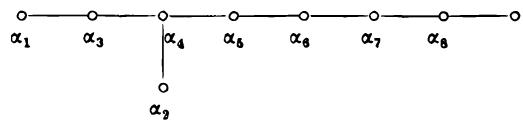
\includegraphics[keepaspectratio]{images/part002_295bff8e.jpg}}

\begin{enumerate}
\def\labelenumi{(\Alph{enumi})}
\setcounter{enumi}{21}
\tightlist
\item
  由于 \((\alpha |\alpha) = 2\) 对所有 \(\alpha \in \mathbb{R}\) 成立，所以 \(R^{\prime} = R\)。
\end{enumerate}

对于 \(\Phi_{\mathrm{R}}\)，根的长度平方为 \(\frac{1}{30}\)（ \(\S 1\)，第 12 号）。因此，\(\Phi_{\mathrm{R}}(x,y) = (x|y)/60\)，且 \(\gamma(\mathrm{R}) = 900\)（ \(\S 1\)，第 12 号，公式 (20)）。

\begin{enumerate}
\def\labelenumi{(\Roman{enumi})}
\setcounter{enumi}{5}
\tightlist
\item
  计算基本权得到
\end{enumerate}

\[
\begin{array}{l} \omega_ {1} = 2 \varepsilon_ {8} = 4 \alpha_ {1} + 5 \alpha_ {2} + 7 \alpha_ {3} + 10 \alpha_ {4} + 8 \alpha_ {5} + 6 \alpha_ {6} + 4 \alpha_ {7} + 2 \alpha_ {8} \\ \omega_ {2} = \frac {1}{2} (\varepsilon_ {1} + \varepsilon_ {2} + \varepsilon_ {3} + \varepsilon_ {4} + \varepsilon_ {5} + \varepsilon_ {6} + \varepsilon_ {7} + 5 \varepsilon_ {8}) \\ \qquad = 5 \alpha_ {1} + 8 \alpha_ {2} + 10 \alpha_ {3} + 15 \alpha_ {4} + 12 \alpha_ {5} + 9 \alpha_ {6} + 6 \alpha_ {7} + 3 \alpha_ {8} \\ \omega_ {3} = \frac {1}{2} (- \varepsilon_ {1} + \varepsilon_ {2} + \varepsilon_ {3} + \varepsilon_ {4} + \varepsilon_ {5} + \varepsilon_ {6} + \varepsilon_ {7} + 7 \varepsilon_ {8}) \\ \qquad = 7 \alpha_ {1} + 10 \alpha_ {2} + 14 \alpha_ {3} + 20 \alpha_ {4} + 16 \alpha_ {5} + 12 \alpha_ {6} + 8 \alpha_ {7} + 4 \alpha_ {8} \\ \omega_ {4} = \varepsilon_ {3} + \varepsilon_ {4} + \varepsilon_ {5} + \varepsilon_ {6} + \varepsilon_ {7} + 5 \varepsilon_ {8} \\ \qquad = 10 \alpha_ {1} + 15 \alpha_ {2} + 20 \alpha_ {3} + 30 \alpha_ {4} + 24 \alpha_ {5} + 18 \alpha_ {6} + 12 \alpha_ {7} + 6 \alpha_ {8} \\ \omega_ {5} = \varepsilon_ {4} + \varepsilon_ {5} + \varepsilon_ {6} + \varepsilon_ {7} + 4 \varepsilon_ {8} \\ \qquad = 8 \alpha_ {1} + 12 \alpha_ {2} + 16 \alpha_ {3} + 24 \alpha_ {4} + 20 \alpha_ {5} + 15 \alpha_ {6} + 10 \alpha_ {7} + 5 \alpha_ {8} \\ \omega_ {6} = \varepsilon_ {5} + \varepsilon_ {6} + \varepsilon_ {7} + 3 \varepsilon_ {8} \\ \qquad = 6 \alpha_ {1} + 9 \alpha_ {2} + 12 \alpha_ {3} + 18 \alpha_ {4} + 15 \alpha_ {5} + 12 \alpha_ {6} + 8 \alpha_ {7} + 4 \alpha_ {8} \\ \omega_ {7} = \varepsilon_ {6} + \varepsilon_ {7} + 2 \varepsilon_ {8} \\ \qquad = 4 \alpha_ {1} + 6 \alpha_ {2} + 8 \alpha_ {3} + 2 \alpha_ {4} + 10 \alpha_ {5} + 8 \alpha_ {6} + 6 \alpha_ {7} + 3 \alpha_ {8} \\ \omega_ {8} = \varepsilon_ {7} + \varepsilon_ {8} \\ \qquad = 5 \alpha_ {1} + 8 \alpha_ {2} + 10 \alpha_ {3} + 15 \alpha_ {4} + 12 \alpha_ {5} + 9 \alpha_ {6} + 6 \alpha_ {7} + 3 \alpha_ {8} = \tilde {\alpha}. \end{array}
\]

\begin{enumerate}
\def\labelenumi{(\Roman{enumi})}
\setcounter{enumi}{6}
\tightlist
\item
  正根之和的一半是基本权之和（§ 1，第 10 号，命题 29）；这给出
\end{enumerate}

\[
\begin{array}{r l} \rho & = \varepsilon_ {2} + 2 \varepsilon_ {3} + 3 \varepsilon_ {4} + 4 \varepsilon_ {5} + 5 \varepsilon_ {6} + 6 \varepsilon_ {7} + 23 \varepsilon_ {8} \\ & = 46 \alpha_ {1} + 68 \alpha_ {2} + 91 \alpha_ {3} + 135 \alpha_ {4} + 110 \alpha_ {5} + 84 \alpha_ {6} + 57 \alpha_ {7} + 29 \alpha_ {8}. \end{array}
\]

\begin{enumerate}
\def\labelenumi{(\Roman{enumi})}
\setcounter{enumi}{7}
\item
  群 \(Q(R)\) 由 \(\varepsilon_{i} \pm \varepsilon_{j}\) 和 \(\frac{1}{2} \sum_{i=1}^{8} \varepsilon_{i}\) 生成，并且等于 \(L_{3}\)（第 4 号）。因此，\(P(R)\)（与 \(Q(R^{\prime}) = Q(R) = L_{3}\) 关联）是 \(L_{3}\)（第 4 号）。连接指标为 1。
\item
  指数族有 8 项，由于 h = 30，与 30 互素的整数 1、7、11、13、17、19、23、29 必须出现在此族中；因此，这些就是 W(R) 的指数。
\item
  由 (IX) 以及第 V 章 § 6 第 2 号命题 3 的推论 1，得到 W(R) 的阶为
\end{enumerate}

\[
2. 8. 12. 14. 18. 20. 24. 30 = 2 ^ {14}. 3 ^ {5}. 5 ^ {2}. 7.
\]

\begin{enumerate}
\def\labelenumi{(\Roman{enumi})}
\setcounter{enumi}{10}
\tightlist
\item
  Dynkin 图的唯一自同构是恒等自同构，因为从分叉点发出的三条链长度各不相同。因此，\(A(R) = W(R)\) 且 \(w_{0} = -1\)。
\end{enumerate}

